\documentclass[xetex,table]{beamer}

\usepackage[autostyle]{csquotes}
\usepackage{hyperref}
\usepackage{color}
\usepackage{setspace}
\usepackage{listings}
\usepackage{minted}

\usetheme{metropolis}

\usemintedstyle{perldoc}

\title{Build Automation:\\Introduzione a Make, Autotools e CMake}
\author{Luca Ceresoli\\
  \href{mailto:luca@lucaceresoli.net}{luca@lucaceresoli.net}\\
  \url{http://lucaceresoli.net}
}
\date{Linux Day 2017}

\begin{document}

\maketitle

\section{Introduzione}

\begin{frame}{Processo di build}
  \begin{center}
    \includegraphics[width=0.7\textwidth]{images/c-example.pdf}

    \pause
    \vspace{0.1\textheight}
    \texttt{gcc -o hello hello.c utils.c}
  \end{center}
\end{frame}

\begin{frame}{Processo di build}
  \begin{flushright}
    \includegraphics[width=0.33\textwidth]{images/c-example.pdf}
  \end{flushright}

  Processo di build:
  \begin{itemize}
  \item Input: il lavoro di un umano
  \item Output: un programma, una libreria, un documento, \dots
  \end{itemize}

  Esempi:
  \begin{itemize}
  \item Codice C / C++ \textrightarrow{} un eseguibile o una libreria
  \item File di testo \textrightarrow{} Un documento PDF
  \end{itemize}
\end{frame}

\begin{frame}{Dove andrà il tuo software domani?}
  \begin{itemize}
  \item Continuous integration / continuous delivery
    \begin{itemize}
    \item Jenkins, Travis CI...
    \item Server locale o ``cloud''
    \end{itemize}
    \pause
  \item Distribuzioni: dpkg, rpm...
    \pause
  \item Sistemi embedded
    \begin{itemize}
    \item Buildroot
    \item Openembedded
    \item OpenWRT
    \end{itemize}
    \pause
  \item Windows, MacOS, Android, iOS
  \end{itemize}
\end{frame}

\begin{frame}{Come vuoi compilare il tuo software?}
  \begin{itemize}
  \item Debug / Release
  \item \texttt{-Wall -Werror}
  \item Librerie: shared / static
  \item \dots
  \end{itemize}
\end{frame}

\begin{frame}{Build automation: necessità}
  \begin{itemize}
  \item Da riga di comando
  \item Deve funzionare in ambienti diversi
  \item Non deve avere {\em policy} hard-coded
  \end{itemize}
\end{frame}

\section{Shell script}

\definecolor{codebackground}{rgb}{0.96,0.96,0.75}

\begin{frame}[fragile]{Shell script semplice}
  \begin{center}
  \includegraphics[height=0.4\textheight]{images/shell.pdf}
  \end{center}

  \texttt{build.sh}:

  \inputminted[bgcolor=codebackground,frame=single]{shell}{examples/1-shell-1/build.sh}
\end{frame}

\begin{frame}{Shell script semplice}
  \begin{itemize}
  \item[\checkmark] Funziona per casi molto semplici
  \item[$\times$]   Ricompila tutto ogni volta (se ci sono 100 file sorgente?)
  \end{itemize}
\end{frame}

\begin{frame}{File oggetto intermedi}
  \center\includegraphics[height=0.5\textheight]{images/depend-graph.pdf}
\end{frame}

\begin{frame}[fragile]{File oggetto intermedi}
  \small\inputminted[bgcolor=codebackground,frame=single]{shell}{examples/1-shell-2/build.sh}
\end{frame}

\begin{frame}{File oggetto intermedi}
  \begin{itemize}
  \item[\checkmark] Più efficiente
  \item[$\times$]   Scomodo da scrivere e mantenere
  \item[$\times$]   Non sfrutta CPU multi core
  \end{itemize}
\end{frame}

\end{document}
